\chapter{低精度分布式更新算法}
本章主要介绍低精度分布式更新(LPDU)算法的实现原理。并详细介绍整个框架工作流程和性能优化的相关方法。通过分析不同应用的理论效率和实际效率结果,评估系统的性能。
\section{引言}
随着人工智能的快速发展,为提升训练效率,满足生产需求,业界已针对分布式深度学习系统进行了深入的研究。本章提出的LPDU算法希望通过低精度数据通信方法来减少分布式同步数据过程中的数据传输量,从而减小同步时间开销,提高分布式训练效率;同时,为保证神经网络的训练精度,本文使用混合精度更新方法对网络进行更新。本章将介绍如何在现有高效的分布式通信框架horovod上集成现有主流的深度学习框架,并进一步实现LPDU算法,分析低精度数据通信相对于原始浮点数通信的缺点,以及对应的改进方法;并介绍相关的优化方法,最后通过理论分析和实验结果比较,说明LPDU算法的有效性和实用性。
\section{MXNet与Horovod的整合}
horovod是uber针对tensorflow在分布式深度学习训练中的不足,基于百度提出的ring-allreduce构建。有3个主要特征:

1. horovod与深度学习框架相互独立,用户以python包的形式调用horovod的API。使其发展独立于任何深度学习框架,目前horovod已经支持tensorflow和pytorch。这样tensorflow和pytorch用户可以在任意版本的深度学习框架中使用horovod,不需要担心兼容问题。目前MXNet团队已经将MXNet整合进了horovod,正在等待horovod团队整合。

2. 用NCCL取代百度ring-allreduce实现。NCCL是NVIDIA的通信库,提供高度优化的ring-allreduce实现。通过NCCL的ring-allreduce实现,使得horovod的性能有巨大提升。

3. 提出tensor fusion方法,通过将多个小的tensor整合成数据量稍大的tensor,进而对这个大的tensor做allreduce。提高了数据的通信效率。

\begin{figure}[htp]
\centering
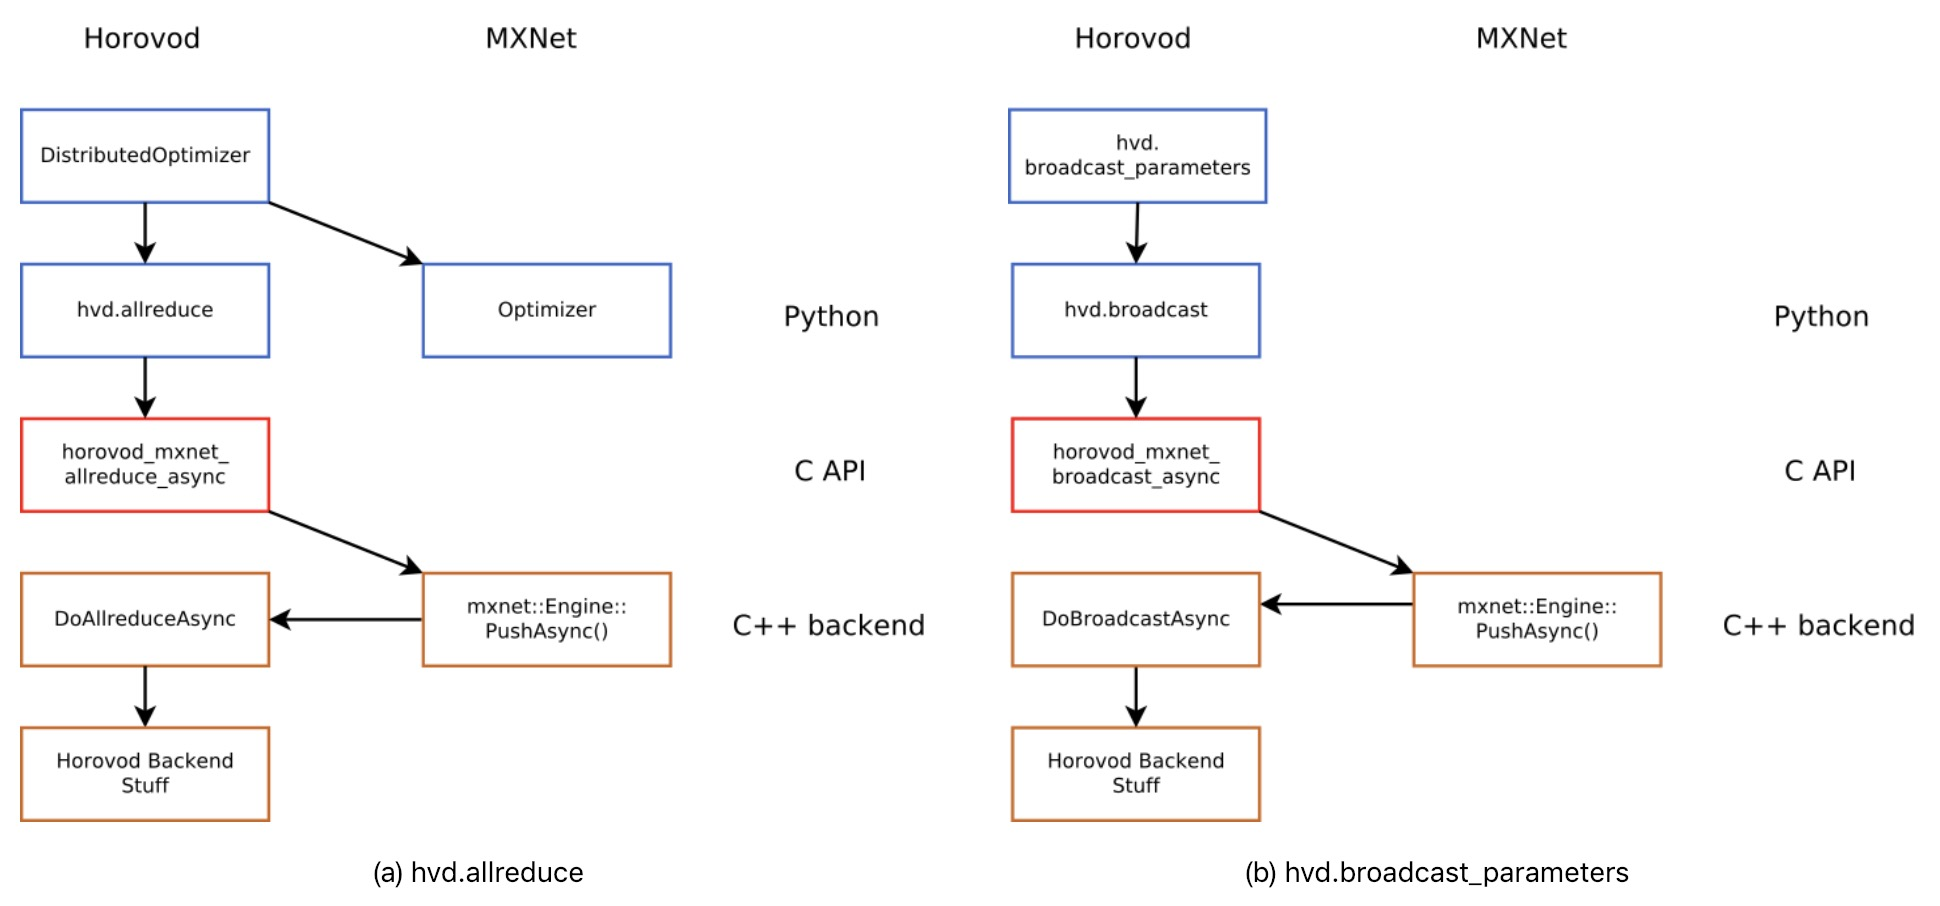
\includegraphics[width=12cm]{horovod_mxnet_integration}
\caption{MXNet与horovod整合示意图}
\label{fig:horovod_mxnet_integration}
\end{figure}
horovod中主要涉及两个操作:allreduce和broadcast。其与MXNet的整合示意图如图~\ref{fig:horovod_mxnet_integration}所示。由图可知,horovod通过继承MXNet的优化器optimizer实现与MXNet的整合,即更新模型时使用horovod的DistributedOptimizer更新。对于MXNet而言,分布式程序只是一个使用DistributedOptimizer优化器更新模型的单机程序。在horovod中,因为其在真正更新之前,会对参数做allreduce来同步全局参数。这种整合方式使得MXNet与horovod可以各自独立发展,而不会产生版本的相互依赖。为保证各个节点中初始化的模型一致, 其提供了一个broadcast parameters的API用于同步模型初始化的值。

horovod通过对外提供tensor接口,各个深度学习框架通过继承该tensor接口,提供自身的实现即可整合到horovod中。接口如下所示:

\begin{lstlisting}[language=C, numbers=none]
Tensor {
  dtype();  //  return the data type of tensor;
  shape();  //  return the shape of tensor;
  data();   //  return the data pointer of tensor;
  size();   //  return the total bytes of data;
}
\end{lstlisting}

由上伪代码可知,将深度学习框架整合进horovod只需通过继承tensor这个基类并实现对应的方法即可。而horovod只需通过调用tensor中的对应方法即可完成数据的同步。故为将MXNet整合入horovod,其设计如下:

\begin{lstlisting}[language=C, numbers=none]
MXTensor : Tensor{
public:
  MXTensor(NDArray* tensor);
  // override the 4 APIs
  dtype();
  shape();
  data();
  size();
protected:
  NDArray* tensor_;  // the pointer address to the data from MXNet
}
\end{lstlisting}

\section{LPDU算法的设计与实现}
LPDU算法主要包含两部分:低精度数据通信和混合精度更新。低精度数据通信部分旨在减少分布式训练过程中的同步通信开销,从而提升分布式训练效率;混合精度更新部分则是为避免低精度数据表示造成的数据精度损失,将同步后的低精度梯度数据转换为原始浮点数,再对网络进行更新,而不是直接使用低精度梯度数据进行更新,减小了更新过程中的数据损失,使用该方法可保证在低精度数据通信情况下神经网络训练精度达到原始浮点数训练的相同精度。
\subsection{低精度数据通信算法}
%分析在训练过程中梯度的分布范围。确定在该范围内,浮点数与bf16数据的精度差距。

由2.1部分可知,相对于单机训练,分布式训练多了额外的同步通信开销,其对分布式训练效率的高低有至关重要的作用。结合业界对低精度数据在神经网络中的研究进展,本节提出一种高效的低精度数据通信方法,在混合精度更新算法配合下,能在不损失神经网络训练精度的情况下,提升分布式训练效率。

算法核心思路是:使用BF16数据格式进行通信,相对于浮点数通信减少了一半数据量,从而提升训练效率。根据业界对低精度数据在神经网络中的研究进展可知,目前主要有两种低精度数据格式用于神经网络训练,分别是半精度浮点数(FP16)和bfloat16(BF16)数据格式。两种在表示数值范围和精度上均有不同程度的损失,通过对应的改进方法,可保证低精度数据下神经网络的训练精度达到原始浮点数训练相同精度。

考虑到FP16与BF16数据格式的特点,BF16数据格式与浮点数之间的转换开销较小,且其可表示的数值范围与浮点数基本相同,故不需要考虑FP16表示情况下梯度数据超过数值表示范围的问题。基于以上两种原因,LPDU算法采用BF16格式数据进行通信,下面介绍基于BF16格式的低精度数据通信算法的具体实现。

基于BF16格式的低精度数据通信算法的实现主要包含两部分:1.在同步之前将原始浮点数转换成BF16格式数据;2.对BF16格式的梯度数据进行同步,求得全局梯度。本文在horovod基础上对低精度数据通信算法进行实现,具体工作包括:1.继承horovod提供的Tensor类,设计BF16 Tensor,供horovod调用,其需要完成原始浮点数到BF16格式数据的转换工作;2.实现一个自定义的BF16求和函数,供MPI在做allreduce过程中对BF16数据求和使用。

针对以上两部分内容,具体设计如下所示。在MXTensor基础上,添加了新的BF16指针,用于存放BF16数据。在构造函数中,将深度学习框架传入的FP32的数据转换成BF16数据。针对第二点BF16的求和函数的实现。因为目前没有BF16的硬件计算单元,求和计算只能在浮点计算单元上计算。由下BF16 sum函数可知,函数主要分为三部分:1.将BF16数据转换为浮点数;2.对浮点数据进行求和;3.将求和后的浮点数结果转换为BF16数据。

\begin{lstlisting}[language=C, numbers=none]
// 1. bf16 tensor defination
MXBF16Tensor: MXTensor {
public:
  MXBF16Tensor(NDArray* tensor):MXTensor(tensor){
  // according the count of tensor elements allocate memory to store bf16 data;
  // convert source data of tensor to bf16 data format
}
  source_data();   // return the source pointer of NDArray;
  // override the 3 APIs as below:
  dtype();  // return bf16 flag;
  data();    // return data pointer of bf16;
  size();     // return the total bytes of bf16 data;
  private:
  unsigned short* bf16dptr_;
}

// 2. implement bf16 sum according MPI_op define
void bf16_sum(void* invec, void* inoutvec, int* len, MPI_Datatype* datatype) {
  for(int i = 0; i < *len; i++) {
    float tmp_in = convert_bf16_to_fp32(invec[i]);
    float tmp_out = convert_bf16_to_fp32(inoutvec[i]);
    tmp_out += tmp_in;
    inoutvec[i] = convert_fp32_to_bf16(tmp_out);
  }
}
\end{lstlisting}


\subsection{混合精度更新算法}
由表1.2可知,BF16格式数据有效数字仅有2~3位,相对于FP32格式数据存在一定精度损失。由随机梯度下降(SGD)更新算法公式3.1可知,SGD将当前梯度乘以学习率$\eta$,再将值更新到模型参数$W$中。通常情况下$\eta$是一个小于0的数,并随着
$$W_{t+1,i}=W_{t,i}-\eta*g_{t,i}$$

为防止数据精度在更新过程中造成进一步的损失,本章提出混合精度更新算法。将同步后的低精度梯度数据转换为浮点数,再使用该浮点梯度数据对模型进行更新。实验证明混合精度更新算法能够保证在低精度数据通信方式下,神经网络的训练精度能达到原始浮点数训练相同精度。


\subsection{LPDU算法设计}
由3.2部分可知,horovod通过继承深度学习框架的优化器实现自定义的分布式优化器DistributedOptimizer达到同步更新的目的。其中DistributedOptimizer的分布式更新算法如算法~\ref{alg:fp32_update}所示。为同步全局梯度,其在调用更新算法之前使用allreduce同步全局梯度,再用全局同步后的梯度更新本地参数,更新后的参数即全局参数。

\begin{algorithm}\small
\caption{原始分布式更新算法}
\textbf{Input:}
本地网络层参数:$Weight$,梯度:$gradient$ \\
\textbf{Output:} 
全局更新后的网络层参数:$Weight$
\begin{algorithmic}[1]
    \STATE{使用$allreduce$对网络层梯度$gradient$做全局同步}
    \STATE{使用更新算法(如随机梯度下降算法),把全局同步后的$gradient$更新到网络层参数$Weight$中}
    \STATE{返回全局更新后的参数$Weight$用于下一次迭代训练}
\end{algorithmic}
	\label{alg:fp32_update}
\end{algorithm}

由第二章介绍可知,BF16计算需要硬件支持,目前只有google的TPU支持该计算,对应地tensorflow对其支持。其他主流框架如pytorch,MXNet则不支持BF16格式的数据类型,故目前BF16只能作为一种数据压缩方式用于分布式深度学习训练中。基于BF16数据同步的分布式更新算法如算法~\ref{alg:bf16_update}所示。为减少数据通信量,其在进行全局同步之前将32比特的梯度数据压缩成了16比特的BF16数据。然后对BF16的数据进行同步,相对于原始32比特的通信方式,该数据通信量减少了一半。在完成全局同步后,再将BF16的梯度转换为32比特的浮点数;最后使用更新算法进行全局更新。

\begin{algorithm}\small
\caption{BF16分布式更新算法}
\textbf{Input:}
本地网络层参数:$Weight$,梯度:$gradient$ \\
\textbf{Output:} 
全局更新后的网络层参数:$Weight$
\begin{algorithmic}[1]
	\STATE{将原始32比特的梯度$gradient$转换为BF16格式的梯度$gradient_{bf16}$}
    \STATE{使用$allreduce$对$gradient_{bf16}$做全局同步}
    \STATE{将全局同步后的梯度$gradient_{bf16}$转换为原始32比特的梯度$gradient$}
    \STATE{使用更新算法(如随机梯度下降算法),把转换后的$gradient$更新到网络层参数$Weight$中}
    \STATE{返回全局更新后的参数$Weight$用于下一次迭代训练}
\end{algorithmic}
	\label{alg:bf16_update}
\end{algorithm}

\subsection{LPDU算法实现}
基于horovod实现BF16数据同步的分布式更新算法主要包含三部分:1.继承horovod提供的Tensor,设计BF16 Tensor供horovod调用;2.实现一个自定义的BF16求和函数,供MPI做allreduce时对BF16数据求和时使用;3.在对BF16做完allreduce后,将BF16数据转换成FP32数据返回给分布式优化器DistriubtedOptimizer进行全局更新。

针对以上三部分内容,具体设计如下所示。在MXTensor基础上,添加了新的BF16指针,用于存放BF16数据。在构造函数中,将深度学习框架传入的FP32的数据转换成BF16数据。针对第二点BF16的求和函数的实现。因为目前没有BF16的硬件计算单元,求和计算只能在浮点计算单元上计算。由下BF16 sum函数可知,函数主要分为三部分:1.将BF16数据转换为浮点数;2.对浮点数据进行求和;3.将求和后的浮点数结果转换为BF16数据。针对第三点,通过在callback函数中添加BF16数据转换到浮点数的过程达到在BF16数据完成allreduce后,将BF16数据转换为FP32数据返回给分布式优化器DistriubtedOptimizer的目的。

\begin{lstlisting}[language=C, numbers=none]
// 1. bf16 tensor defination
MXBF16Tensor: MXTensor {
public:
  MXBF16Tensor(NDArray* tensor):MXTensor(tensor){
  // according the count of tensor elements allocate memory to store bf16 data;
  // convert source data of tensor to bf16 data format
}
  source_data();   // return the source pointer of NDArray;
  // override the 3 APIs as below:
  dtype();  // return bf16 flag;
  data();    // return data pointer of bf16;
  size();     // return the total bytes of bf16 data;
  private:
  unsigned short* bf16dptr_;
}

// 2. implement bf16 sum according MPI_op define
void bf16_sum(void* invec, void* inoutvec, int* len, MPI_Datatype* datatype) {
  for(int i = 0; i < *len; i++) {
    float tmp_in = convert_bf16_to_fp32(invec[i]);
    float tmp_out = convert_bf16_to_fp32(inoutvec[i]);
    tmp_out += tmp_in;
    inoutvec[i] = convert_fp32_to_bf16(tmp_out);
  }
}

// 3. convert bf16 data to fp32 data on callback function.
void callback() {
        // convert bf16_tensor to fp32, assign to output
        mxnet.tensor.dptr = BF16ToFloat(bf16_pointer, len);
        handle_manager.MarkDone(handle);
        handle_manager.ExecuteCallback(handle);
      }
\end{lstlisting}

\subsection{性能优化}
为减小FP32数据与BF16数据的转换开销,提高BF16 sum中计算效率,我们通过使用intrinsic指令直接操作数据完成数据转换和计算,达到SSE汇编代码相同的性能效果。针对不同情况,进行了最优实现。考虑到部分数据地址并不符合AVX512指令地址对齐要求,故需要额外使用movdqu指令处理数据地址不对齐的情况。下面分别是在数据地址满足AVX512指令地址要求和不满足其地址要求情况下,浮点数据转换到bf16数据的具体实现。同理,BF16数据转换到浮点数和BF16 sum中的相关计算与之类似。

\begin{lstlisting}[language=C, numbers=none]
// 数据不对齐情况:使用movdqu指令处理
inline void convert_f32_to_b16(const void* src, void* dst)
{
  __m512i y = _mm512_bsrli_epi128(_mm512_loadu_si512(src), 2);
  _mm256_storeu_si256((__m256i*)(dst), _mm512_cvtepi32_epi16(y));
}

// 数据对齐情况:直接使用intrinsic指令计算
inline void convert_f32_to_b16(__m512i* src, __m256i* dst)
{
  __m512i y = _mm512_bsrli_epi128(*src, 2);
  *dst = _mm512_cvtepi32_epi16(y);
}
\end{lstlisting}

考虑到不同硬件对intrinsic指令对支持程度,本文分别BF16更新算法中设计的每种操作进行了三种实现:naive,AVX256,AVX512以兼容不同硬件。如表~\ref{tab:intrinsic_perf}所示。可知相对于原始实现方法,AVX512实现有2.2~5.7倍的性能提升;AVX256实现有1.6~3.4倍的性能提升。

\begin{longtable}[c]{c*{6}{l}}
\caption{不同实现下性能加速比}\label{tab:intrinsic_perf}\\
\toprule[1.5pt]
 功能函数 & 数组大小 & 
\multicolumn{1}{c}{原始实现} & \multicolumn{1}{c}{AVX512实现} &
\multicolumn{1}{c}{AVX256实现} & \multicolumn{1}{c}{AVX512} & 
\multicolumn{1}{c}{AVX256} 	\\
\multicolumn{1}{c}{} &\multicolumn{1}{c}{} &\multicolumn{1}{c}{(us)} & \multicolumn{1}{c}{(us)} &
\multicolumn{1}{c}{(us)} & \multicolumn{1}{c}{speedup} &
\multicolumn{1}{c}{speedup} 	\\

\midrule[1pt]%
\endfirsthead%

\multicolumn{7}{c}{续表~\thetable\hskip1em 不同实现下性能加速比}\\

\toprule[1.5pt]
 功能函数 & 数组大小 & 
\multicolumn{1}{c}{原始实现} & \multicolumn{1}{c}{AVX512实现} &
\multicolumn{1}{c}{AVX256实现} & \multicolumn{1}{c}{AVX512} & 
\multicolumn{1}{c}{AVX256} 	\\
\multicolumn{1}{c}{} &\multicolumn{1}{c}{} &\multicolumn{1}{c}{(us)} & \multicolumn{1}{c}{(us)} &
\multicolumn{1}{c}{(us)} & \multicolumn{1}{c}{speedup} &
\multicolumn{1}{c}{speedup} 	\\
\midrule[1pt]%
\endhead%
\hline%

\multicolumn{7}{r}{续下页}%

\endfoot%
\endlastfoot%
F32ToBF16 &	100 & 0.297 & 0.117 & 0.148 & 2.552 & 2.010  \\
F32ToBF16 &	1000 & 2.309 & 0.480 & 0.736 & 4.812 & 3.137  \\
F32ToBF16 &	10000 & 22.612 & 3.923 & 6.183 & 5.763 & 3.657  \\
F32ToBF16 &	100000 & 216.404 & 41.076 & 63.768 & 5.268 & 3.394 \\
F32ToBF16 &	1000000 & 2039.863 & 374.645 & 586.142 & 5.445 & 3.480 \\
BF16ToF32 &	100 & 0.279 & 0.109 & 0.169 & 2.549 & 1.649 \\
BF16ToF32 &	1000 & 2.117 & 0.442 & 0.986 & 4.794 & 2.147 \\
BF16ToF32 &	10000 & 20.492 & 3.795 & 9.129 & 5.400 & 2.245 \\
BF16ToF32 &	100000 & 267.662 & 103.113 & 158.061 & 2.596 & 1.693 \\
BF16ToF32 &	1000000 & 2715.713 & 1188.977 & 1658.944 & 2.284 & 1.637 \\
BF16 sum &	100 & 0.456 & 0.200 & 0.314 & 2.285 & 1.453 \\
BF16 sum &	1000 & 3.993 & 1.089 & 2.528 & 3.665 & 1.579 \\
BF16 sum &	10000 & 39.258 & 9.740 & 23.867 & 4.031 & 1.645 \\
BF16 sum &	100000 & 404.553 & 113.089 & 253.198 & 3.577 & 1.598 \\
BF16 sum &	1000000 & 3898.513 & 981.624 & 2390.526 & 3.971 & 1.631 \\
\bottomrule[1.5pt]
\end{longtable}

\section{实验与分析}
为说明BF16分布式更新算法的有效性,本节将从神经网络的训练性能和精度两方面进行对比分析。同时,为了说明BF16更新算法的普适性,我们将分别展示图像分类、物体检测等领域网络在BF16更新算法下的效果。为验证BF16分布式更新算法的高效性,本节将单独比较原始分布式更新算法与BF16分布式更新算法的效率。同时对实验细节和数据集也进行了详细介绍,使得实验结果和分析更具说服力。

\subsection{数据集介绍}
为说明本章提出的BF16更新算法的广泛适用性。本章分别从典型的图像分类、物体检测应用中选择代表的神经网络在各自领域公开数据集上进行实验,分别与原始训练结果进行对比,验证BF16分布式更新算法的有效性。数据集信息如表~\ref{tab:datasets}所示。

ILSVRC2012: ImageNet数据集,包含1281167张图片,1000个类别,总容量约140GB,是图像分类领域公认的权威数据集。

PASCAL VOC: 为图像识别和分类提供了一整套标准化数据。本文使用其2007与2012年发布的数据集,用于训练物体检测网。包含16551个有效物体框,共20个类别,总容量约2.8GB。

\begin{table}[htbp]
\centering
\begin{minipage}[t]{0.9\linewidth}
\caption{数据集概况}
\label{tab:datasets}
\begin{tabularx}{\linewidth}{l X X X }
\toprule[1.5pt]
{\song 数据集名称} & {\song 适用场景} & {\song 样本数量} & {	\song 类别数量}\\
\midrule[1pt]
ILSVRC2012 & 图像分类 & 1281167 & 1000\\
VOC2007+2012 & 目标检测 & 16551 & 20\\
\bottomrule[1.5pt]
\end{tabularx}
\end{minipage}
\end{table}

\subsection{实验环境介绍}
本文使用MXNet 1.3版本,在ctcyang/horovod:mxnet feature fp16分支基础上进一步设计实现BF16更新算法。所有实验均在双sockets的Xeon Gold 6148处理器的集群中运行所得结果。因为目前各个框架CPU端计算性能均基于单socket进行优化。在每个socket上跑一个训练实例可使训练效率达到最佳。故本文在每个机器节点上跑两个训练实例,使得每个socket上跑一个训练实例,以充分发挥CPU计算性能。

\subsection{BF16分布式更新算法性能分析}
由3.3部分算法分析可知,BF16更新算法开销包含四部分时间开销:通信时间、FP32数据转换BF16数据开销、对BF16数据求和开销、BF16数据转换为FP32数据开销;原始更新算法开销包含两部分时间开销:通信开销与FP32数据求和开销。在不同数据规模下,测得8节点16实例实验环境中原始更新算法与BF16更新算法时间开销如下表~\ref{tab:fp32_bf16_update_time}所示。可知在数据量大于10000时,BF16更新算法相对于原始更新算法有加速。随着数据量的增大,加速效果越明显;当数据量增大到1000000时,BF16更新算法加速比能达到1.35,可以预测数据量越大,通信开销占比越大,BF16更新算法加速比也将进一步增大。

\begin{table}[htbp]
  \centering
  \caption{不同数据规模下两种更新算法时间开销}
  \label{tab:fp32_bf16_update_time}
  \begin{minipage}[t]{0.8\textwidth} 
    \begin{tabularx}{\linewidth}{|l|X|X|X|}
      \hline
      数组大小  & FP32 alg$^{*}$(us) & BF16 alg$^{**}$(us) & Speedup\\
      \hline
100 & 6842.00 & 6332.42 & 1.08 \\
1000 & 5213.00 & 5216.59 & 1.00 \\
10000 & 6317.00 & 6204.70 & 1.02 \\
100000 & 7245.00 & 6081.76 & 1.19 \\
1000000 & 20668.00 & 15259.92 & 1.35 \\
      \hline
    \end{tabularx}\\[2pt]
    \footnotesize
    *:原始分布式更新算法时间开销:通信和浮点数求和时间\\
    **:BF16分布式更新算法时间开销:FP32ToBF16,BF16ToFP32,通信和BF16求和时间
  \end{minipage}
\end{table}

本节以50层的resnet网络为例,从理论上分析该网络在8节点16训练实例环境中,BF16更新算法相对于原始更新算法的理论性能收益。 由表~\ref{tab:resnet50_params}可知,仅有2.8\%的参数的数据规模小于100000,97.2\%参数的规模均大于100000,64.57\%参数的规模大于1000000。根据表~\ref{tab:fp32_bf16_update_time}数据可知:在50层的resnet网络中,BF16更新算法相对于原始更新算法的更新时间将有1.19~1.35倍的加速,甚至大于1.35倍的加速。

\begin{table}[htbp]
\centering
\begin{minipage}[t]{0.9\linewidth}
\caption{resnet50各层参数大小分布}
\label{tab:resnet50_params}
\begin{tabularx}{\linewidth}{l X X }
\toprule[1.5pt]
{\song 参数规模} & {\song 参数个数} & {\song 占比(\%)}\\
\midrule[1pt]
<100000 & 713920 & 2.80 \\
100000-1000000 & 8323072 & 32.63 \\
>1000000 & 16466920 & 64.57 \\
\bottomrule[1.5pt]
\end{tabularx}
\end{minipage}
\end{table}

在50层resnet网络的真实训练场景中,原始更新算法与BF16更新算法在不同训练实例个数的更新时间如表~\ref{tab:fp32_bf16_real_update_time}所示。在8节点16实例情况下,BF16更新算法相对于原始更新算法的更新时间有1.3倍的性能提升,在8节点情况下同步时间由原始的0.458s降低至0.352s,可节省30\%的更新时间。与表~\ref{tab:fp32_bf16_update_time}和上述分析1.19~1.35倍的性能提升相一致。两者相互验证,说明了算法实现的正确性和有效性。 

\begin{table}[htbp]
  \centering
  \caption{不同训练实例中两种算法更新时间$^{*}$}
  \label{tab:fp32_bf16_real_update_time}
  \begin{minipage}[t]{0.8\textwidth} 
    \begin{tabularx}{\linewidth}{|l|X|X|X|X|}
      \hline
      节点数 & 实例数 & FP32 alg(s) & BF16 alg(s) & Speedup\\
      \hline
1 & 1 & 0.015 & 0.041 & 0.366 \\
1 & 2 & 0.075 & 0.076 & 0.987 \\
2 & 4 & 0.374 & 0.299 & 1.251 \\
4 & 8 & 0.428 & 0.337 & 1.270 \\
8 & 16 & 0.458 & 0.352 & 1.301 \\
      \hline
    \end{tabularx}\\[2pt]
    \footnotesize
    *:训练配置:resnet50,每个训练实例batch size=128\\
  \end{minipage}
\end{table}

为进一步比较原始更新算法与BF16更新算法在实际训练过程中的性能差异,本节通过采样得到不同训练实例下,实际训练中每次迭代时间如表~\ref{tab:fp32_bf16_real_iter_time}所示。可知在8节点16训练实例情况下,BF16更新算法的单次迭代时间相对于原始更新算法减少了0.12s,其来自于BF16算法同步时间的降低。该时间与表~\ref{tab:fp32_bf16_real_update_time}中同步时间减少部分相一致。因为BF16算法降低了同步时间开销,使得分布式训练效率相对于原始更新算法有所提升。如在8节点16训练实例情况下,BF16更新算法使得分布式训练效率由84.05\%提升至87.5\%,提升了3.5个百分点。不可否认,现阶段CPU训练神经网络速度远慢于GPU训练,使得分布式训练中通信压力相对较小。若使用GPU训练,单次迭代中计算时间将大大减少,使得同步时间占比增大。此时BF16更新算法对提升分布式训练效率的作用将更加明显。

\begin{table}[htbp]
  \centering
  \caption{不同训练实例中两种算法迭代时间}
  \label{tab:fp32_bf16_real_iter_time}
  \begin{minipage}[t]{0.8\textwidth} 
    \begin{tabularx}{\linewidth}{|l|X|X|X|X|X|}
      \hline
      节点数 & 实例数 & FP32 time & BF16 time & FP32 & BF16 \\
       &  & (s/iter) & (s/iter) & scaling & scaling\\
      \hline
1 & 1 & 2.8158 & 2.8271 & 100.00 & 100.00 \\
1 & 2 & 2.8685 & 2.9990 & 98.16 & 94.27 \\
2 & 4 & 3.0450 & 3.0387 & 92.47 & 93.04 \\
4 & 8 & 3.3332 & 3.1877 & 84.48 & 88.69 \\
8 & 16 & 3.3501 & 3.2310 & 84.05 & 87.50 \\
      \hline
    \end{tabularx}\\[2pt]
  \end{minipage}
\end{table}

由上述分析可知,神经网络的参数量越大,受网络带宽限制,同步开销越大,BF16更新算法对分布式性能提升作用越大。同时,该算法普遍适用于各种主流神经网络,如图像分类,物体检测和递归循环网络等。表~\ref{tab:ssd_vgg_scaling}分别展示了BF16更新算法在物体检测网络SSD和分类网VGG中的性能提升。可知模型稍小的SSD网络中,BF16更新算法可使分布式训练效率由85.01\%提升至89.84\%,相对于原始更新算法提升了4.83个百分点;在模型较大的VGG网络中该算法性能提升更加明显,相对于原始FP32更新算法,在8节点16训练实例情况下提升了7.13\%。
\begin{table}[htbp]
  \centering
  \caption{原始更新算法与BF16更新算法在SSD与VGG网络中的性能加速}
  \label{tab:ssd_vgg_scaling}
  \begin{minipage}[t]{0.8\textwidth} 
    \begin{tabularx}{\linewidth}{|l|X|X|X|X|}
      \hline
      实例数 & SSD$^{*}$ FP32 & SSD BF16 & VGG$^{**}$ FP32 & VGG BF16 \\
       & scaling & scaling & scaling & scaling\\
      \hline
1 & 100.00 & 100.00 & 100.00 & 100.00 \\
2 & 96.88 & 97.81 & 88.78 & 92.17 \\
4 & 91.97 & 95.18 & 86.65 & 90.06 \\
8 & 88.44 & 92.27 & 83.48 & 89.44 \\
16 & 85.01 & 89.84 & 79.42 & 86.55 \\
      \hline
    \end{tabularx}\\[2pt]
    \footnotesize
    *:SSD的模型大小为101MB\\
    **:VGG的模型大小为528MB
  \end{minipage}
\end{table}

\subsection{BF16分布式更新算法精度比较}
为说明BF16更新算法不会对神经网络精度造成影响,本节分别比较在相同配置下,原始更新算法和BF16更新算法下神经网络最终的收敛精度。图~\ref{fig:resnet50_4node_acc}为4节点8实例情况下原始FP32更新算法与BF16更新算法的收敛曲线。可知在训练集与验证集上BF16算法均与原始FP32更新算法的精度曲线基本重合,最终精度也保持一致,说明BF16更新算法在分类网中不会造成网络的精度损失。不同节点实例下原始更新算法与BF16更新算法在ImageNet数据集上的最终结果如表~\ref{tab:resnet50_diff_node_acc}所示。可知相同节点数下,BF16更新算法与原始更新算法下收敛精度差距不超过0.3\%,该细微误差属于网络训练过程中的正常波动。说明不同节点下BF16更新算法均能保证神经网络的训练精度收敛到理想精度,验证了BF16更新算法的有效性与正确性。

\begin{figure}[htp]
\centering
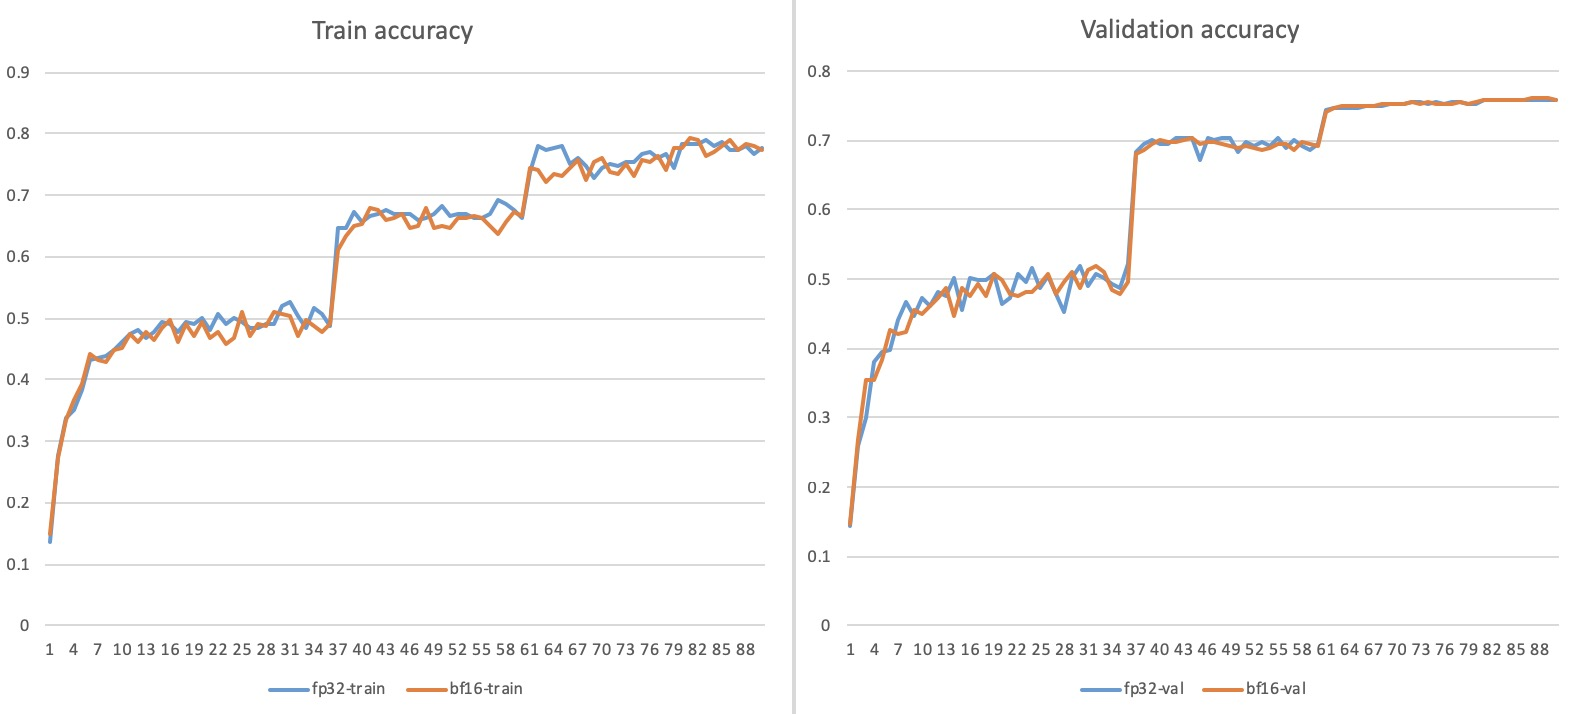
\includegraphics[width=13cm]{resnet50_4node_acc2}
\caption{resnet50中原始更新算法与BF16更新算法收敛曲线}
\label{fig:resnet50_4node_acc}
\end{figure}

\begin{table}[htbp]
\centering
\begin{minipage}[t]{0.9\linewidth}
\caption{resnet50在不同节点数下最终精度}
\label{tab:resnet50_diff_node_acc}
\begin{tabularx}{\linewidth}{l X X X }
\toprule[1.5pt]
{\song 数据集} & {\song 节点数} & {\song FP32更新算法(\%)} & {	\song BF16更新算法(\%)}\\
\midrule[1pt]
ILSVRC2012 & 1 &  76.18 & 76.15\\
ILSVRC2012 & 4 & 76.20 & 75.98\\
ILSVRC2012 & 8 & 76.08 & 76.13\\
\bottomrule[1.5pt]
\end{tabularx}
\end{minipage}
\end{table}
为验证BF16更新算法对神经网络的普遍适用性,本节以物体检测领域经典网络SSD为例,使用BF16更新算法对其进行训练,通过比较原始更新算法与本文算法在验证集的收敛曲线和最终收敛结果验证BF16算法的有效性。如图~\ref{fig:ssd_4node_acc}所示:在4节点8实例情况下,BF16更新算法与原始更新算法在验证集上的mAP曲线基本重合,说明BF16更新算法在物体检测网络中不会造成网络的精度损失。不同节点实例下原始更新算法与BF16更新算法在VOC数据集上的最终结果如表~\ref{tab:ssd_diff_node_acc}所示,可知相同节点数下,BF16更新算法与原始更新算法下验证集结果差距不超过0.4\%,在正常数据波动范围内。该误差来源于神经网络正常训练误差和BF16数据造成的部分数据损失。说明不同节点情况下BF16更新算法均能保证神经网络的训练精度收敛到原始FP32更新算法相接近的精度,验证了BF16更新算法的有效性与正确性。 

\begin{figure}[htp]
\centering
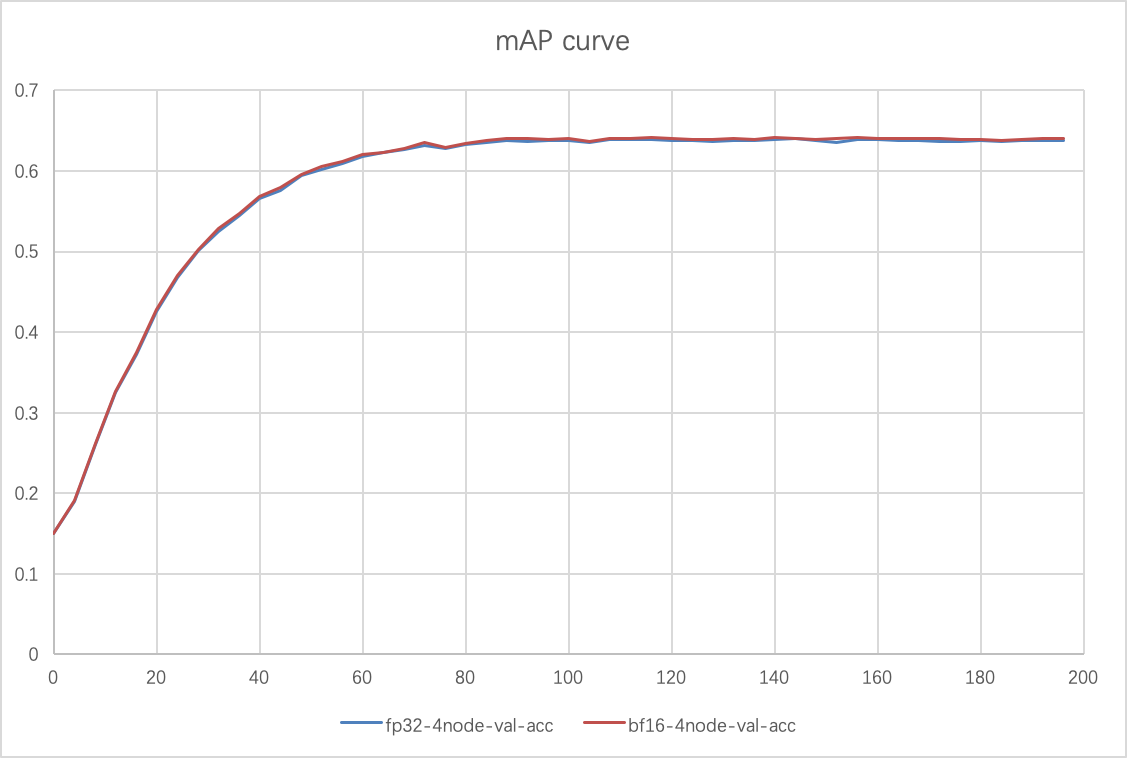
\includegraphics[width=10cm]{ssd_4node_acc}
\caption{SSD中原始更新算法与BF16更新算法收敛曲线}
\label{fig:ssd_4node_acc}
\end{figure}


\begin{table}[htbp]
\centering
\begin{minipage}[t]{0.9\linewidth}
\caption{ssd在不同节点数下最终精度}
\label{tab:ssd_diff_node_acc}
\begin{tabularx}{\linewidth}{l X X X }
\toprule[1.5pt]
{\song 数据集} & {\song 节点数} & {\song FP32更新算法(\%)} & {	\song BF16更新算法(\%)}\\
\midrule[1pt]
VOC2007+2012 & 1 & 64.22 & 64.18\\
VOC2007+2012 & 4 & 64.00 & 64.06\\
VOC2007+2012 & 8 & 64.04 & 63.64\\
\bottomrule[1.5pt]
\end{tabularx}
\end{minipage}
\end{table}

\section{本章小结}
本章主要提出了BF16分布式更新算法以减小分布式训练过程中同步时间的开销,提升了分布式训练神经网络的效率。首先介绍了将horovod整合进MXNet的设计原理,并进一步在此基础上介绍了BF16分布式更新算法的设计与实现,以及BF16更新算法实现过程中优化性能的相关方法。最后对BF16更新算法中各个模块的时间开销进行了详细分析,验证本章算法的高效性。最后将该算法用于训练分类网和物体检测网,通过比较BF16更新算法与原始更新算法的训练效率与神经网络最终的收敛精度,说明了本章算法在不影响神经网络训练精度情况下,使得分布式训练效率有明显提升。也说明了BF16更新算法对神经网络的普遍适用性。
